\chapter{Espacios topológicos}
\label{cha:espacios_topologicos}
La primera parte de este manual pretende hacer un estudio formal de la definición de la estructura de espacio topológico. Uno de los objetivos de esta noción es, por ejemplo, desvincular los conceptos topológicos como son abiertos, cerrados, fronteras, etc. de las propiedades métricas en $\mathbb{R}^n$. Fundamentalmente, esto servirá para poder estudiar características como continuidad, convergencia, conexión... en espacios más enrevesados y, como añadido, estudiar estas propiedades en espacios ya conocidos, pero con una estructura asociada distinta.

\section{Conjuntos abiertos}
\label{sec:conjuntos_abiertos}
Al igual que en el Álgebra Lineal la parte más básica y fundamental eran los vectores, vamos a ver que en la topología las piezas claves son los abiertos. Estos son los que nos permiten dar forma y definir el resto nociones del capítulo. Además, el conjunto de abiertos en un conjunto es el que caracteriza y diferencia las topologías con las que pueda ser equipado este entre sí.

\begin{defi}[Espacio Topológico]
Sea $X$ un conjunto de elementos que denotaremos por \textbf{puntos} y $\mathcal{T} \subset \mathcal{P}\left( X \right)$ una colección de subconjuntos que denotaremos \textbf{abiertos}, decimos que $\mathcal{T}$ es una \textbf{topología} de $X$ si y sólo si:
\begin{enumerate}
    \item $\emptyset, X \in \mathcal{T}$ 
    \item $\bigcup_{i \in I} U_i \in \mathcal{T}$ donde $U_i \in \mathcal{T}$
    \item $\bigcap_{i=1}^n U_i \in \mathcal{T}$ donde $U_i \in \mathcal{T}$
\end{enumerate}
y, ese caso, la dupla $\left( X, \mathcal{T} \right)$ se denomina \textbf{espacio topológico}.
\end{defi}

\begin{ej}
\begin{enumerate}
    \item \textbf{Topología trivial}: \label{ejemplos_topologia:first}
    
    La topología es $\mathcal{T} = \{\emptyset, X\}$ para cualquier conjunto $X$ sobre el que se equipe. Es la topología con menos abiertos posibles y esto hace que esté contenida en cualquier otra topología.
    \item \textbf{Topología discreta}:
    
    La topología es $\mathcal{T} = P\left( X \right)$ para cualquier conjunto $X$ sobre el que se equipe. Es la topología con más\footnote{Porque si los puntos $\{x\} \in X$ son abiertos, entonces cualquier conjunto $A = \bigcup_{x \in A} \{x\}$ es abierto.} abiertos posibles y esto hace que cualquier otra esté contenida en ella.
    \item \textbf{Topología usual}:
    
    Si al conjunto $\mathbb{R}^n$ le equipamos la topología en las que los abiertos son los conjuntos formados por unión de bolas euclídeas, obtenemos la topología habitual que utilizamos en $\mathbb{R}^n$.
    
    \item Cualquier distancia $d(x,y)$ define una topología a través de sus bolas abiertas, igual que definíamos la usual en $\mathbb{R}^n$, de hecho, se puede demostrar sin mayor dificultad (y tal y como se ve en el dibujo) que todas las normas $p$ en $\mathbb{R}^n$ definen bolas que contienen y están contenidas en las restantes. En consecuencia, si la definición de abierto usual se hacía a través de bolas redondas y hemos visto que estas contienen a bolas cuadradas o romboidales, también se tiene que es abierto cuadrado o romboidal y el recíproco por los contenidos en ambos lados.
    \begin{figure}[H]
        \centering
        \incfig[0.7]{normas-topología}
        \caption{\textit{El dibujo representa distintas topologías generadas por distintas normas, pero todas equivalentes.}}
        \label{fig:normas-topología}
    \end{figure}

    Es decir, cambiar de norma igual cambia la noción de distancia en $\mathbb{R}^n$, ¡pero no la topología asociada! Sigue siendo la topología usual de $\mathbb{R}^n$.
    
    \item \textbf{Topología del punto}:
    
    La topología es $\mathcal{T}_a := \{U \subset X: a \in U\} \cup \{\emptyset\}$ para un $a\in X$ fijado previamente. Lo curioso de esta topología es que todos los abiertos son los conjuntos que contienen a $a\in X$, es decir, que la topología queda caracterizada como $\mathcal{T}_a := \{{a, W} \text{ donde }W\subset X\}$.
\end{enumerate}
\end{ej}

\begin{defi}[Entorno]
Sea $(X, \mathcal{T})$ un espacio topológico y $x\in X$ un punto del mismo, definimos un \textbf{entorno\footnote{Cuando el abierto que contiene al punto es el propio entorno o, dicho de otra manera, el entorno de $x$ es un abierto de la topología, decimos que es un entorno \textit{abierto} de $x$.} del punto $x$} como un conjunto $V^x$ que contiene un abierto $U$ que contiene al punto:
\[
V^x := V\subset X : \exists U \subset V \text{ donde }x\in U
\]
\end{defi}

%TODO: Mejorar imagen
\begin{figure}[H]
    \centering
    \incfig[0.6]{definición-entornos}
    \caption{\textit{Definición de entornos}}
    \label{fig:definición-entornos}
\end{figure}

\begin{prop}[Caracterización de abierto]
Sea $(X, \mathcal{T})$ un espacio topológico y $W \subset X$ un subconjunto de puntos, este es abierto si y sólo si es entorno de todos sus puntos.
\end{prop}
\begin{demo}
La implicación de izquierda a derecha es trivial, pues todo conjunto se contiene a sí mismo y, como el conjunto es abierto, contiene a un abierto que contiene al punto, es decir, es entorno de cualquiera de sus puntos.

Para probar el recíproco, si un subconjunto $W\subset X$ es entorno de todos sus puntos, entonces para cada $x$ del conjunto existe un $U^x\subset W$ que contiene a $x$. Por tanto, podemos expresar $W$ como unión arbitraria de todos estos abiertos, es decir, $W = \bigcup_{x\in W} U^x$ y, por ser topología, la unión arbitraria de abiertos es abierta.
\end{demo}

\begin{prop}
Sea $(X,\mathcal{T})$ un espacio topológico y $V_1^x$ y $V_2^x$ dos entornos de un punto $x\in X$, entonces la intersección $V^x := V_1^x\cap V_2^x$ es entorno de $x$.
\end{prop}
\begin{demo}
Por definición de entornos, existen dos abiertos $U_1^x\subset V_1^x$ y $U_2^x\subset V_2^x$ que contienen a $x$. Por la definición de topología, la intersección finita $U^x := U_1^x\cap U_2^x$ es un abierto de la topología y vemos que $U^x \subset V^x$, luego $V^x$ contiene a un abierto que contiene al punto, es decir, es entorno.
\end{demo}

\begin{defi}[Punto interior]
Sea $(X,\mathcal{T})$ un espacio topológico y $A \subset X$ un subconjunto de puntos, decimos que un punto $x\in X$ es \textbf{punto interior de $A$} si y sólo si $A$ es entorno de $x$.
$$
x\in \inter_X(A) \Leftrightarrow \exists U \ab A : x \in U
$$
Al conjunto de puntos interiores, que denotamos por $\mathring{A}$ o $\inter(A)$, lo llamamos \textbf{interior de $A$}.
\end{defi}

%TODO: Mejorar bordes
\begin{figure}[H]
    \centering
    \incfig[0.6]{definición-interior}
    \caption{\textit{Definición de interior de un conjunto.}}
    \label{fig:definición-interior}
\end{figure}

\begin{prop}
Sea $A\subset X$ un subconjunto de puntos, entonces:
\begin{itemize}
\item $\mathring{A}$ es el mayor abierto en $A$ o, lo que es lo mismo, $ \mathring{A} = \bigcup_{U \subset A} U$.
\item $A$ abierto si y sólo si todos sus puntos son interiores, es decir, $A = \mathring{A}$
\end{itemize}
\end{prop}
\begin{demo}
\begin{enumerate}
    \item Si $x\in \mathring{A}$, entonces $\exists U \subset A : x\in U \Rightarrow x\in \bigcup_{U\subset A}U$, pero es que si $x\in U$ para algún $U\subset A$, por definición es interior de $A$, luego $x\in \mathring{A}$.
   
   Como $\mathring{A}$ es unión de abiertos, la definición de topología nos asegura que será un abierto y además es el más grande de todos porque cualquier otro está contenido en él por ser la unión de todos los abiertos.   
   \item El contenido $\mathring{A}\subset A$ se tiene siempre, puesto que $x\in \mathring{A}\Leftrightarrow \exists U \subset A : x\in U \subset A \Rightarrow x\in A$ (dicho de otra forma, los puntos interiores de $A$ son aquellos para los cuales $A$ es entorno y como un entorno contiene al punto se tiene trivialmente).
   
   De esta manera, si $A$ es abierto, como $\mathring{A}$ es el mayor abierto de $A$, tiene que ser $\mathring{A} = A$ y si $\mathring{A} = A$, como $\mathring{A}$ es abierto, pues lo es $A$.
\end{enumerate}
\end{demo}

\begin{ej}
\begin{enumerate}
    \item Si consideramos un espacio topológico $\left( X, \mathcal{T}_{\text{trivial}} \right)$ con la discreta, vemos que cualquier subconjunto $A\subset X$ puede contener únicamente a $\emptyset$ como abierto, luego su interior es el vacío $\mathring{A} = \emptyset$.

    \item Si consideramos $(\mathbb{R}^n, \mathcal{T}_{\text{usual}})$ algunos de los interiores usuales son $\inter\left( B\left[ a, \varepsilon \right] \right)  = B\left( a, \varepsilon \right)$, $\mathring{\mathbb{Q}}^n = \emptyset$ y $\mathring{\mathbb{Z}}^n = \emptyset$.
    
    \item Si consideramos la topología del punto $\mathcal{T}_a$, entonces $\mathring{\{a\}} = \{a\}$ y, en general, ocurre lo mismo para cualquier conjunto que contenga a $a$ (porque son abiertos). Sin embargo, cualquier $x \neq a$ verifica que $\mathring{\{x\}} = \emptyset$.
\end{enumerate}
\end{ej}

\begin{coro}
\begin{enumerate}
    \item $A \subset B \Rightarrow \mathring{A} \subset \mathring{B}$.
    \item $\mathring{A} \cap \mathring{B} = \inter \left( A \cap B \right)$.
\end{enumerate}
\end{coro}
\begin{demo}
\begin{enumerate}
    \item La relación $A \subset B \Rightarrow \mathring{A} \subset A \subset B$ implica que, como $\mathring{A}$ es abierto y $\mathring{B}$ es la unión de todos los abiertos de $B$, $\mathring{A} \subset \mathring{B}$.
    \item En primer lugar, como $\mathring{A}\cap \mathring{B}$ es intersección de abiertos, entonces es abierto y está contenido en $A\cap B$, luego por ser $\inter(A\cap B) = \bigcup_{U\in A\cap B}U$ sabemos que $\mathring{A}\cap \mathring{B} \subset \inter(A\cap B)$.
    
	Recíprocamente, si $x\in \inter(A\cap B)$ existe un abierto $U \in A\cap B$ tal que $x\in U$. Por ser de la intersección, en particular también es abierto de cada conjunto, luego $x\in \mathring{A}$ y $x\in \mathring{B}$, es decir, $x\in \mathring{A}\cap \mathring{B}$.
\end{enumerate}
\end{demo}

\section{Conjuntos cerrados}%
\label{sec:conjuntos_cerrados}
Los conjuntos cerrados por definición están íntimamente relacionados con los conjuntos abiertos. Revisten gran importancia por la relación que tienen con dos conjuntos de puntos importantes: la acumulación y la adherencia. Estas dos últimas nociones permiten caracterizar conceptos como la convergencia de sucesiones o la densidad de un conjunto.

\begin{defi}[Conjunto cerrado]
Sea $\left( X, \mathcal{T} \right)$ un espacio topológico y $F\subset X$ un subconjunto de puntos, decimos que es un \textbf{conjunto cerrado} si y sólo si su complementario es un abierto, es decir, $U = X \setminus F$ es abierto.
\end{defi}

\begin{obs}
En muchas ocasiones el lenguaje natural confunde las definiciones precisas que se dan en matemáticas. Este caso es un ejemplo de ello: uno podría pensar que la definición de cerrado desprende el hecho de que un cerrado es un ``no abierto''. Sin embargo, podemos encontrar multitud de conjuntos que no ni abiertos ni cerrados
\begin{figure}[H]
    \centering
    \incfig[0.5]{observación-abiertos-y-cerrados.}
    \caption{\textit{Ejemplo de conjunto que no es ni abierto ni cerrado.}}
    \label{fig:observación-abiertos-y-cerrados.}
\end{figure}
e incluso otros que son abiertos y cerrados simultáneamente, como el vacío y el total.
\end{obs}

\begin{prop}
Sea $(X,\mathcal{T})$ un espacio topológico y denotando por $\mathcal{F}$ al conjunto de cerrados del espacio, entonces:
\begin{enumerate}
    \item $\emptyset, X \in \mathcal{F}$.
    \item $\bigcap_{i \in I} F_i \in \mathcal{F}$ donde $F_i \in \mathcal{F}$.
    \item $\bigcup_{i=1}^n F_i \in \mathcal{F}$ donde $F_i \in \mathcal{F}$.
\end{enumerate}
\end{prop}
\begin{demo}
\begin{itemize}
\item Trivial, porque el uno es el complementario del otro y ambos son abiertos.

\item Porque el complementario de la intersección $X\setminus \left(\bigcap_{i \in I} F_i \right) = \bigcup_{i \in I} \left( X \setminus F_i \right) = \bigcup_{i \in I} U_i$ es abierto.

\item Porque el complementario de la unión $X\setminus \left(\bigcup_{i = 0}^n F_i\right) = \bigcap_{i=0}^n \left( X \setminus F_i\right) = \bigcap_{i=0}^n U_i$ es abierto.
\end{itemize}
\end{demo}

\begin{ej}
\begin{enumerate}
    \item \textbf{Topología trivial}:
    
    En este caso, como $\emptyset$ y $X$ son los únicos abiertos, únicamente pueden ser cerrados sus complementarios, es decir, ellos mismos.
    
    \item \textbf{Topología usual}:
    
	Habitualmente los conjuntos que conocemos como cerrados son aquellos que pueden ser escritos en términos de bolas cerradas $B\left[ a, \varepsilon \right] : \lVert x - a \rVert \le \varepsilon$.
	
    \item Si tenemos dos topologías $\mathcal{T}_1 \subset \mathcal{T}_2$, entonces cualquier cerrado de $\mathcal{T}_1$ es cerrado de $\mathcal{T}_2$, pues es cerrado por ser el complementario de un abierto y los abiertos de $\mathcal{T}_1$ también lo son el $\mathcal{T}_2$.
\end{enumerate}
\end{ej}

\begin{defi}[Adherencia]
Sea $A \subset X$ y $x\in X$ un punto, decimos que es \textbf{adherente a $A$} si y sólo si todos sus entornos $V^x$ intersecan con $A$, esto es:
$$
\adh_X\left( A \right) = \overline{A} := \{x \in X: \forall V^x \cap A \neq \emptyset\} \supset A
$$
Al conjunto de puntos adherentes a $A$ lo llamamos \textbf{adherencia} de $A$.
\end{defi}

\begin{obs}
La propia definición nos sugiere ciertas equivalencias útiles que se obtienen escribiendo de forma distinta lo que hemos definido:
\begin{itemize}
\item $X \setminus \overline{A} = \inter\left( X \setminus A \right)$
$$
x \in X \setminus \overline{A} \Leftrightarrow x \not\in \overline{A} \Leftrightarrow \exists U^x \cap A = \emptyset \Leftrightarrow \exists U^x \subset X \setminus A \Leftrightarrow x \in \inter\left( X \setminus A \right)
$$
\item $X \setminus \mathring{B} = \overline{X \setminus B}$
$$
x \not\in \mathring{B} \Leftrightarrow \nexists U^x \subset B \Leftrightarrow \forall U^x \cap \left( X \setminus B \right) \neq \emptyset \Leftrightarrow x \in \overline{X \setminus B}
$$
\end{itemize}
\end{obs}

\begin{prop}
Sea $A\subset X$ un subconjunto de puntos y denotando por $\overline{A}$ a su adherencia, entonces:
\begin{itemize}
\item $\overline{A}$ es el menor cerrado que contiene a $A$ o, lo que es lo mismo, $\overline{A} = \bigcap_{F \supset A} F$ donde los $F$ son cerrados.

\item El conjunto $A$ es cerrado si y sólo si coincide con su adherencia, es decir, $\overline{A} = A$.

\item $B \subset A \Rightarrow \overline{B} \subset \overline{A}$.
\item $\overline{A \cup B} = \overline{A} \cup \overline{B}$.
\end{itemize}
\end{prop}
\begin{demo}
\begin{itemize}
\item Recordando que $\mathring{B} = \bigcup_{U \subset B} U$:
$$
\overline{A} = X \setminus \inter\left( X \setminus A \right) = X \setminus \left(\bigcup_{U \subset X \setminus A} U \right) \stackrel{F = X \setminus U}{=} X \setminus \left(\bigcup_{F \supset A} \left( X \setminus F \right) \right) = \bigcap_{F \supset A} F
$$
\item Se deduce inmediatamente de la primera, pues si el conjunto es cerrado él mismo debe ser el menor cerrado que lo contiene.
\item Si $B \subset A \Rightarrow$
$$
B \subset A \subset \overline{A} \Rightarrow \overline{B} \subset \overline{A}
$$
por el primer apartado.
\item Veamos el doble contenido:
$$
\begin{cases}
	\overline{A\cup B} \supset A \cup B \supset
		A,B \Rightarrow \overline{A\cup B} \supset
		\overline{A}, \overline{B} \Rightarrow \overline{A\cup B} \supset \overline{A} \cup \overline{B} \\
	A \cup B \subset \overline{A} \cup \overline{B} \Rightarrow \overline{A\cup B} \subset \overline{A} \cup \overline{B}
\end{cases} \Rightarrow \overline{A}\cup \overline{B} = \overline{A\cup B}
$$
\end{itemize}
\end{demo}

\begin{ej}
\begin{enumerate}
    \item En $\mathbb{R}^n, \mathcal{T}_{\text{usual}}: B\left[ a, \varepsilon \right] = \overline{B \left( a, \varepsilon \right)};\ \overline{\mathbb{Q}^n} = \mathbb{R}^n$.
    \item Sea $a \in X$ con $\mathcal{T}_a \Rightarrow$
    \begin{itemize}
        \item $\overline{\{a\}} = X $
        \begin{demo}
            $\forall x, \forall U^x \supset \{a, x\} \ni a \Rightarrow x \in \overline{\{a\}}$
        \end{demo}
        \item $\forall x \neq a, \overline{\{x\}} = \{x\}$
        \begin{demo}
            $y \neq x \Rightarrow U^y = \{a, y\} \cap \{x\} = \emptyset$ 
        \end{demo}
    \end{itemize}
\end{enumerate}
\end{ej}

\begin{defi}[Acumulación]    
Sea $A\subset X$ un subconjunto de puntos y $x\in A$ un punto del mismo, decimos que $x$ es:
\begin{itemize}
\item \textbf{punto aislado de $A$} si y sólo si existe algún entorno que sólo interseca con $A$ en el propio punto, es decir:
$$
\exists V^x \subset X : V^x \cap A = \{x\}
$$
\item \textbf{punto de acumulación de $A$} si y sólo si en cualquier entorno del punto encontramos puntos de $A$ que no sean el propio punto, es decir:
$$
\forall V^x \subset X : V^x \cap A \setminus \{x\} \neq \emptyset
$$
\end{itemize}
\end{defi}

\begin{obs}
La definición anterior para puntos aislados hace evidente el hecho de que los puntos aislados solo pueden ser de $A$. Por contra, los puntos de acumulación no tienen por qué y, de hecho, su definición en términos de entornos prescinde de ellos mismos para analizar su intersección con $A$. De esta manera, obtenemos el siguiente resultado:
$$
\overline{A} = \{\underbrace{\text{puntos aislados}}_{\subset A}\} \sqcup \{\underbrace{\text{puntos de acumulación}}_{\supset \overline{A} \setminus A}\}
$$
Además, nótese que si uno es punto de $A$ sólo tiene dos posibilidades: ser aislado o ser de acumulación. Por tanto, podemos reescribir lo anterior como:
$$
\overline{A} = A \cup A'
$$
\end{obs}

\begin{defi}[Frontera]
Sea $A\subset X$ un subconjunto de puntos y $x\in A$ un punto del mismo, decimos que $x$ es un \textbf{punto frontera de $A$} si y sólo si es adherente\footnote{Por las observaciones hechas sobre las adherencias, también podríamos caracterizar los puntos frontera como los que no son interior de $X \setminus A$ ni de $A$.} a $A$ y a su complementario $X \setminus A$
    \[
    \fr\left( A \right) := \overline{A} \cap \overline{X \setminus A} = \overline{A} \setminus \mathring{A}     
    \]
al conjunto de puntos de la frontera de $A$ lo llamamos \textbf{frontera} de $A$.
\end{defi}

\begin{ej}
\begin{enumerate}
    \item En $\mathbb{R}$, con la topología usual $\mathcal{T}_u$, todos los puntos de $\mathbb{Z}$ son aislados. Por tanto, la frontera de los enteros es $\fr\left( \mathbb{Z} \right) = \mathbb{Z}$.
    \item En $\mathbb{R}^n$, con la topología usual $\mathcal{T}_u$, la frontera de las bolas $\fr\left( B\left( a, \varepsilon \right) \right) = \fr\left( B\left[ a, \varepsilon \right] \right) = S\left[ a, \varepsilon \right] : \lVert x - a \rVert = \varepsilon$ son los discos exteriores de las mismas.
    \item En la topología $\mathcal{T}_{\text{discreta}}$, sobre cualquier conjunto que se equipe, todos los puntos son aislados y, en consecuencia, todas las fronteras, vacías.
    \item En la topología del punto $\mathcal{T}_a$ sobre un punto $a \in X$ concreto vemos que:
$$
\begin{cases}
	\fr\left( \{a\} \right) = \overline{\{a\}} \setminus \mathring{\{a\}} = X \setminus \{a\} \\
    x \neq a \Rightarrow \fr\left( \{x\} \right) = \overline{\{x\}} \setminus \mathring{\{x\}} = \{x\} 
\end{cases} 
$$
\end{enumerate}
\end{ej}

\begin{defi}[Densidad]
Sea $X$ un conjunto de puntos y $A \subset X$ un subconjunto suyo, decimos que $A$ es \textbf{denso en $X$} si y sólo si $\overline{A} = X$ o, dicho de otro modo, todo abierto no vacío corta a $A$.
\end{defi}

\begin{ej}
\begin{enumerate}
    \item En $\mathbb{R}$, con la topología usual $\mathcal{T}_u$, el conjunto de los números racionales $\mathbb{Q} \subset \mathbb{R}$ es denso en $\mathbb{R}$.
    \item En la topología del punto $\mathcal{T}_a$, el conjunto $\{a\}$ es denso, pues cualquier abierto corta con él (lo contiene).
\end{enumerate}
\end{ej}

\section{Bases}%
\label{sec:bases}
En general, probar una cierta propiedad para una topología hace necesario verificar dicha propiedad en todos los abiertos de la misma. Esto, ya de por sí complicado, puede serlo mucho más cuando la definición de abierto es compleja y poco intuitiva. Por esto, del mismo modo que en el Álgebra Lineal surgían las bases para trabajar con un espacio vectorial completo observando únicamente un conjunto pequeño de vectores, en Topología tendremos las bases de entornos y de abiertos que jugaran un papel similar en los espacios topológicos.

\begin{defi}[Base de entornos]
Sea $(X, \mathcal{T})$ un espacio topológico y $a\in X$ un punto, definimos una \textbf{base de entornos de $a \in X$} como una colección $\mathcal{V}^a$ de entornos de $a$ tales que cualquier otro entorno de $a$ tenga que contener a alguno de los entornos de la colección $\mathcal{V}^a$, esto es:
\[
\forall W^a, \ \exists V \in \mathcal{V}^a : V \subset W^a
\]
\end{defi}

\begin{obs}
La definición no ha hecho ninguna diferenciación especial en cuanto a si son cerrados, abiertos, etc. Precisamente esta ``variedad'' es la que permite que, escogiendo una base de entornos con las características adecuadas en cada caso, sea más sencillo estudiar la topología que tengamos entre manos.

Tal y como hemos comentado al inicio, comprobar propiedades en una base de entornos extenderá automáticamente dichas propiedades a cualquier entorno arbitrario, haciendo el estudio de estos conjuntos más sencillos en función de la topología y la base escogida.
\end{obs}

\begin{prop}
Sea $(X,\mathcal{T})$ un espacio topológico y $\{V_i^a \}_{i\in I}$ una base de entornos de un punto $a$, esta se puede refinar a una base de entornos abiertos $\{U_i^a\}_{i\in I}$. 
\end{prop}
\begin{demo}    
Como todos los elementos de la colección son entornos, para todos existe algún abierto $U_i^a$ que contiene al punto. A este conjunto de abiertos (más bien de entornos abiertos) es al que llamamos $\{U_i^a\}_{i\in I}$. Cualquier otro entorno del punto $a$ contiene a un entorno $V_i^a$ de la base de entornos inicial, pero como estos contienen un abierto de la colección última, entonces $\{U_i^a\}_{i\in I}$ es una base de entornos de  $a$.
\end{demo}

\begin{obs}    
Podemos empezar a ver la utilidad de la base de entornos cuando tenemos que demostrar, por ejemplo, que un punto pertenece a la adherencia de un conjunto:
$$
a \in \overline{A} \xLeftrightarrow{\text{def.}} \forall W^a \text{ entorno}: W^a \cap A \neq \emptyset \Leftrightarrow \forall V^a \in \mathcal{V}^a: V^a\cap A \neq \emptyset
$$
luego si escogemos una base de entornos $\mathcal{V}^a$ adecuada sobre la que sea muy fácil demostrar el resultado, este quedará demostrado para cualquier entorno ``raro'' que podamos encontrarnos.
\end{obs}

\begin{ej}
\begin{enumerate}
    \item Sea el espacio real usual $(\mathbb{R}^n, \mathcal{T}_{\text{usual}})$ el espacio topológico a estudiar, entonces:
    $$
    \begin{cases}
    \mathcal{B}^a = \{B\left( a, \varepsilon \right): \varepsilon > 0\} \text{ base de entornos abiertos.}  \\
    \mathcal{V}^a = \{B\left[ a, \varepsilon \right]: \varepsilon > 0\} \text{ base de entornos cerrados.} 
    \end{cases} 
    $$
    \item Sea la topología del punto $(a \in X, \mathcal{T}_a)$, entonces:
	$$
	\begin{cases}
	\mathcal{B}^a = \{\{a\}\} & x = a\\
	\mathcal{B}^x = \{\{a, x\}\} & x \neq a
	\end{cases}
	$$
\end{enumerate}
\end{ej}

\begin{defi}[Base de abiertos]
Sea $(X, \mathcal{T})$ un espacio topológico y $\mathcal{B} :=\{U_i\}_{i\in I}\subset \mathcal{T}$ una colección de abiertos, decimos que es una \textbf{base de abiertos de $\mathcal{T}$} si y sólo si todo abierto de $\mathcal{T}$ es unión de abiertos de $\mathcal{B}$.
\end{defi}

\begin{prop}[Caracterización de base de abiertos]
Sea $(X, \mathcal{T})$ un espacio topológico y $\mathcal{B} :=\{U_i\}_{i\in I}\subset \mathcal{T}$ una colección de abiertos, los siguientes enunciados son equivalentes:
\begin{enumerate}
\item $\mathcal{B}$ es base de abiertos. 
\item $\forall x \in X, \ \mathcal{B}^x = \left\{ B \in \mathcal{B} : x \in B \right\}$ es base de entornos de $x$.
\item $\forall x \in U \ab X, \ \exists B \in \mathcal{B} : x \in B \subset U$.
\end{enumerate}
\end{prop}

\begin{demo}
La implicación $2. \Rightarrow 3.$ es trivial, pues si $U$ es abierto y contiene al punto es un entorno del mismo, luego por $2.$ debe contener a alguna $B\in \mathcal{B}$. Por tanto, demostraremos $1. \Rightarrow 2.$ y $3. \Rightarrow 1.$ para completar las equivalencias.
\begin{itemize}
\item $1. \Rightarrow 2.$

Si $V^x$ es entorno, entonces $\exists U \subset V^x$ abierto que contiene al punto $x$. Como por $1.$ el conjunto $B$ es base de abiertos, $U = \bigcup_{B_i \in \mathcal{B}} B_i$ y como $x\in U$, entonces $\exists B_i \ni x$. De esta manera, tenemos $B_i \subset U \subset V^x$, es decir, que cualquier entorno debe contener algún elemento de la base que contenga al punto.

\item $3. \Rightarrow 1.$

Por darse $3.$, escogido cualquier abierto $U$ necesariamente contiene a una $B^x\in \mathcal{B}$ para cada $x\in U$, es decir, que podemos escribir $U = \bigcup_{x \in U} B^x$ unión de abiertos de $\mathcal{B}$.
\end{itemize}
\end{demo}

\begin{ej}
\begin{enumerate}
    \item Si tomamos la topología discreta $\mathcal{T}_{\text{discreta}}$ entonces una base de abiertos sería $\mathcal{B} = \{\{x\} : x \in X\}$. Además, esta base es mínima pues cualquier otra base $B' := \{B_i\}_{i\in I}$ de abiertos cumpliría que $\forall x  : \{x\} = \bigcup_{i \in  I} B_i \Rightarrow \exists i \in I : B_i = \{x\}$.
    \item Si tomamos la topología del punto $\mathcal{T}_a$, entonces una base de abiertos es $\mathcal{B} = \{\{a, x\} : x \in X\}$.
    \item Si tomamos la topología usual $\mathbb{R}^n, \mathcal{T}_{\text{usual}}$ en $\mathbb{R}^n$, entonces una base de abiertos es el conjunto de bolas abiertas $\mathcal{B} = \{B\left( x, \varepsilon \right) : \varepsilon > 0 \mbox{ y } x \in \mathbb{R}^n\}$ porque recordemos que un abierto se caracterizaba en $\mathbb{R}^n$ por el hecho de que todos sus puntos tenían una bola alrededor contenida en el conjunto, luego la unión de dichas bolas es el abierto inicial.
    Sin embargo, la base de abiertos lo sigue siendo si escogemos otra norma en $\mathbb{R}^n$ distinta de la euclídea, puesto que estas normas eran equivalentes en $\mathbb{R}^n$ (o, visto geométricamente, cada bola de una norma contiene otra más pequeña de otra norma distinta y viceversa)
    porque
    \[
    B\left( x, \varepsilon \right) = \bigcup_{i \in  I} \ooalign{$\sqsubset\mkern3mu$\cr$\mkern3mu\sqsupset$\cr}_i = \bigcup_{j \in J} \diamond_i
    \]
\begin{figure}[H]
    \centering
    \incfig[0.4]{bases-alternativas-en-rn}
    \caption{\textit{Bases alternativas en $\mathbb{R}^n$}}
    \label{fig:bases-alternativas-en-rn}
\end{figure}
\end{enumerate}
\end{ej}

% TODO: no me convencen estos entornos y el de ilustración habría que cambiarlo por proposición.
\begin{pg}
    Como antes, a menudo basta considerar los abiertos de $\mathcal{B}$. 
\end{pg}

\begin{il}
$A \subset X$ denso $\Leftrightarrow \forall B \in \mathcal{B}, B \cap A \neq \emptyset$.
\end{il}

\begin{prop}
Sea $X$ un conjunto de puntos y $\mathcal{B} := \left\{ B_i \right\}_{i \in I} \subset \mathcal{P}\left( X \right)$ una colección de subconjuntos, esta colección define una topología $\mathcal{T}$ única en $X$ si y sólo si: 
\begin{itemize}
    \item $X = \bigcup_{i\in I} B_i$.
    \item $\forall B_i,B_j\in \mathcal{B} \mbox{ y } \forall x \in B_i \cap B_j, \ \exists B_k \in \mathcal{B} : x\in B_k\subset B_i \cap B_j$.
\end{itemize}
\begin{figure}[H]
    \centering
    \incfig[0.6]{caracterización-de-la-topología-dada-una-base}
    \caption{\textit{Caracterización de la topología dada una base}}
    \label{fig:caracterización-de-la-topología-dada-una-base}
\end{figure}

\end{prop}
%TODO: Mejorar
\begin{demo}
\begin{itemize}
\item[$\Rightarrow)$]

Trivial por las propiedades vistas sobre topología.

\item[$\Leftarrow)$]

Veamos que se verifican las condiciones sobre la topología:
\begin{itemize}
    \item \textbf{Unicidad}: $\mathcal{T} = \{\bigcup_{i \in  I} B_i: \{B_i\} \subset \mathcal{B}\}$.
    \item \textbf{Existencia}: Esa $\mathcal{T}$ es efectivamente topología. 
        \begin{itemize}
            \item $\emptyset \in \mathcal{T}$, $X = \bigcup_{i\in I} B_i \in \mathcal{T}$.
            \item Uniones: $\bigcup_{j\in J} \left(\bigcup_{i\in I} B_{i}\right) = \bigcup_{j\in J} B_{ij} \in \mathcal{T}$. 
            \item Intersecciones finitas: $B_1, B_2 \in \mathcal{B} \Rightarrow B_1 \cap B_2 = \bigcup_{x \in B_1 \cap B_2} B^x \in \mathcal{T}$.
            $$
            x \in \left( \bigcup_{i} B_i \right) \cap \left( \bigcup_{k} B_k \right) \Rightarrow x \in B_{i_0} \cap B_{k_0} \Rightarrow \exists B^x \in \mathcal{B} : x\in B^x \subset B_{i_0} \cap B_{k_0}
            $$
            Por tanto, podemos decir que $\left( \bigcup_{i} B_i \right) \cap \left( \bigcup_{k} B_k \right) = \bigcup_{x} B^x \in \mathcal{T}
            $ y se tiene el resultado.
        \end{itemize}
\end{itemize}
\end{itemize}
\end{demo}

\section{Topología relativa}%
\label{sec:topologia_relativa}
De la misma manera que en Álgebra, una vez definida la estructura de espacio vectorial, estudiábamos como se comportaba esta estructura con los subconjuntos del conjunto inicial, tiene sentido preocuparnos por cómo cambia la topología cuando nos restringimos a un subconjunto de puntos del total. A esta topología ``restringida'' la conocemos como topología relativa y, a diferencia de lo que ocurría en espacios vectoriales, puede tener un comportamiento muy distinto a la topología ambiente de la que proviene.

\begin{defi}[Topología Relativa]
Sea $\left( X, \mathcal{T} \right)$ un espacio topológico e $Y \subset X$ un subconjunto de puntos, definimos la \textbf{topología relativa\footnote{La comprobación de que efectivamente se trata de una topología es completamente trivial.} en $Y$} como
$$
\mathcal{T}|_Y = \{U \cap Y: U \in \mathcal{T}\}
$$
Además, decimos que $\left( Y, \mathcal{T}|_Y \right)$ es un \textbf{subespacio} de $\left( X, \mathcal{T} \right)$ y que $\left( X, \mathcal{T} \right)$ es el espacio \textbf{ambiente}. 
\end{defi}
%TODO: Mejorar
\begin{figure}[H]
    \centering
    \incfig[0.6]{definición-topología-relativa.}
    \caption{\textit{Definición de una topología relativa}}
    \label{fig:definición-topología-relativa}
\end{figure}

\begin{obs}
\begin{enumerate}
    \item Los cerrados de la topología relativa $\mathcal{T}|_Y$ son la intersección $F\cap Y$ de $Y$ con cerrados $F$ en $\mathcal{T}$.
    \begin{demo}
    Sea $F \cerr Y \Rightarrow$
    \begin{align*}
    F &= Y\setminus W : W \ab Y \Rightarrow \exists U \ab X : Y\cap U = W\\    
    &\Rightarrow F = Y \setminus (Y \cap U) = Y \cap  (X\setminus U) = Y \cap F_x : F_x \cerr X
    \end{align*}
    \end{demo}

    \item Si tenemos una base $\mathcal{V}^a$ de entornos en el espacio ambiente $(X,\mathcal{T})$, la base de entornos en el subespacio $(Y,\mathcal{T}|_Y)$ se obtiene intersecando los elementos de la base ambiente con el subespacio, es decir, $\mathcal{V}^a_Y := \mathcal{V}^a \cap Y := \{V^a \cap Y : V^a \in \mathcal{V}^a\}$.

    \item Si tenemos una base $\mathcal{B}$ de abiertos en el espacio ambiente $(X,\mathcal{T})$, la base de abiertos en el subespacio $(Y,\mathcal{T}|_Y)$ se obtiene intersecando\footnote{Esta idea suele ser general, las construcciones en los subespacios se hacen intersecando elementos del espacio ambiente con el subespacio.} los elementos de la base ambiente con el subespacio, es decir, $\mathcal{B}_Y := \mathcal{B} \cap Y := \{B \cap Y : B \in \mathcal{B}\}$.
\end{enumerate}
\end{obs}


\begin{ej}
\begin{enumerate}
    \item Si $y$ es un punto aislado de $Y$, por la definición que hemos dado de la topología relativa, su topología relativa sería $\mathcal{T}|_Y := \{ U \cap \{y\} \} = \{y\}$. Por tanto, es abierto en su topología.
    
    \item Retomando el ejemplo anterior, si todos los puntos de $Y$ son aislados, hemos visto que todos son abiertos (pues cortar un abierto con ellos da ellos mismos) y, por tanto, la topología $\mathcal{T}|_Y $ es la discreta. Por ejemplo, en $\mathbb{Z} \subset \mathbb{R}$:
\begin{figure}[H]
    \centering
    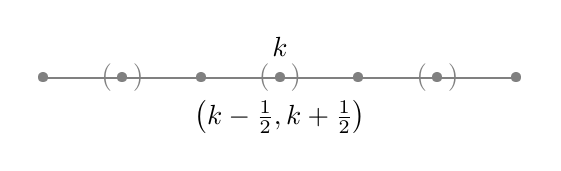
\begin{tikzpicture}
        \draw[gray] (-3,0) -- (3,0);
        \foreach \Point in {(-3, 0), (-2, 0), (-1, 0), (0, 0), (1, 0), (2, 0), (3, 0)}{
            \node[gray] at \Point {\textbullet};
        }
        \foreach \Point in {(-2.2, 0), (-0.2, 0), (1.8, 0)}{
            \node[gray] at \Point {$($};
        }
        \foreach \Point in {(-1.8, 0), (0.2, 0), (2.2, 0)}{
            \node[gray] at \Point {$)$};
        }
        \node at (0, 0.4) {$k$};
        \node at (0, -0.5) {$\left( k - \frac{1}{2}, k + \frac{1}{2} \right)$};
    \end{tikzpicture}
    \caption{\textit{Enteros en los reales como subespacio discreto.}}
    \label{fig:enteros-en-los-reales-como-subespacio-discreto.}
\end{figure}

    \item Si tomamos la topología del punto $(a \in X, \mathcal{T}_a|_{X \setminus \{a\}})$ vemos que se trata de la discreta.
\end{enumerate}
\end{ej}

\begin{obs}
\begin{enumerate}
    \item Los abiertos $W$ de un subespacio abierto $Y \ab X$ son abiertos en el espacio ambiente $X$.
   	$$
    W = U \cap Y : U,\ Y\ab X \Rightarrow W \ab X 
    $$
    \item Los cerrados $F$ de un subespacio cerrado $Y \cerr X$ son cerrados en el espacio ambiente $X$.
    $$
    F = C \cap Y : Y,\ C\cerr X \Rightarrow F \cerr X
    $$
\end{enumerate}
\end{obs}

